\documentclass{article}

\usepackage{hyperref}

\usepackage{epstopdf}
\usepackage{amsmath}
\usepackage{amssymb}
\usepackage{subfig}
%\usepackage{multirow}
\usepackage[utf8]{inputenc}
\usepackage[T1]{fontenc}
\usepackage{standalone}
\usepackage{tikz}
\usepackage{tabularx}

\graphicspath{{img/}}
\DeclareGraphicsExtensions{.pdf,.png,.jpg} %For pdflatex

\begin{document}



% Uwaga! Standardowo pdflatex nie obsługuje plików jp2 i gif. Obsługiwane są m.in formaty: png, jpeg i pdf
% wystarcza to do zamieszczania grafik dowolnego typu:
% pdf: grafika wektorowa,
% jpg: obrazy rzeczywiste,
% png: inne rodzaje grafiki rastrowej.
% Ważne, że w pliku pdf osadzane są dokładnie te pliki, które przygotowaliśmy bez dodatkoweh rekompresji czy  skalowania
% - czyli jeśli dodajemy do dokumentu plik o rozmiarze 100kB to wynikowy pdf powiększy się o ten rozmiar, doatkowo grafika 
% nie ulegnie degradacji.
%
%
% W ćwiczeniu dotyczących formatów grafiki, aby pokazać efekty kompresji jp2 i gif, wystarczy zapisać prezentowane 
% wycinki w bezstratnym formacie png. Co jest pokazane w tym przykładzie.

% Poniżej grafiki umieszczone za pomocą polecenia subfloat w ukaładzie 3 kolumny 2 wiersze:


\newcommand{\ww}{0.3} %zmienna używana jako parametr opisujące szerokość obrazu zdefiniowana poraz pierwszy w dokumencie

\begin{figure}
%
\captionsetup[subfloat]{position=bottom,labelformat=empty} %
\subfloat[BMP: size=x~kB; PNG: PSNR=INF, size=x2~kB]{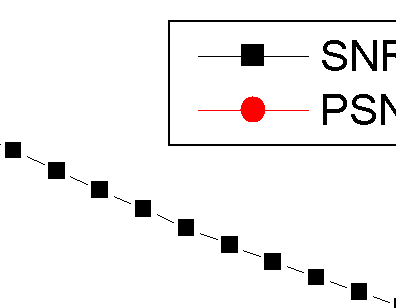
\includegraphics[width=\ww\linewidth]{obraz1}}
\hfill%	
\subfloat[GIF: PSNR=x~dB, size=s~kB]{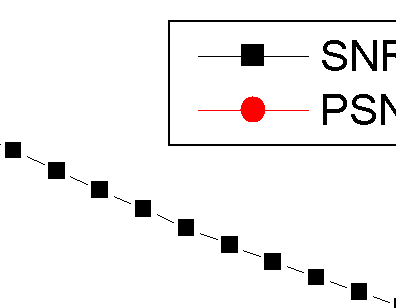
\includegraphics[width=\ww\linewidth]{obraz1_gif}} %oczywiście w tym przypadku gifa nie trzeba zamieszczać bo jest identyczny jak png i bmp, możecie go pominąć lub wstawić pusty element1
\hfill% wypełnenie
\subfloat[JPG: q=1, PSNR=x1~dB, size=s~kB]{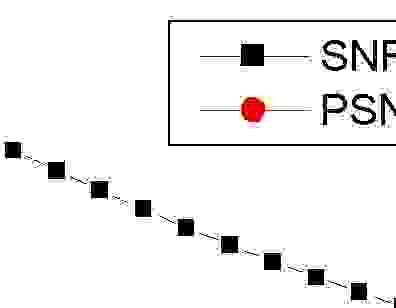
\includegraphics[width=\ww\linewidth]{obraz1_q=1.jpg}}
\hfill
\subfloat[JPG: q=80, PSNR=x1~dB, size=s~kB]{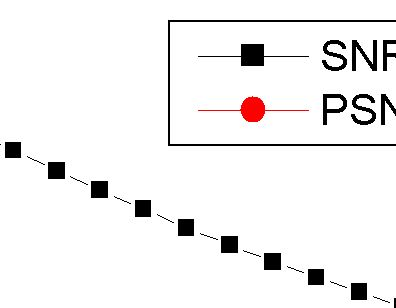
\includegraphics[width=\ww\linewidth]{obraz1_q=80.jpg}}
\hfill%
\subfloat[JP2: Q=8, PSNR=x~dB, size=s~kB]{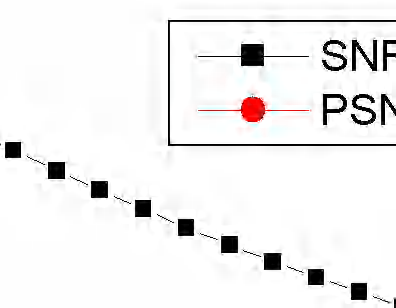
\includegraphics[width=\ww\linewidth]{obraz1_Q=8_jp2}}
\hfill%
\subfloat[JP2: Q=30, PSNR=x~dB, size=s~kB]{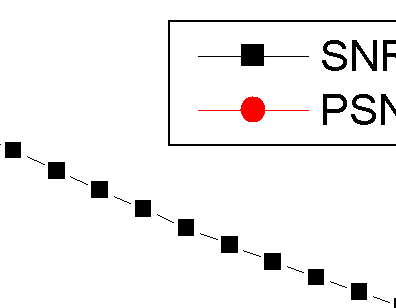
\includegraphics[width=\ww\linewidth]{obraz1_Q=30_jp2}}
\caption{Porównanie metod kompresji dla obrazu syntetycznego} %
\label{fig:porownanie1} %label który można wykorzystać w tekście za pomocą polecenia \ref{fig:porownanie1}
\end{figure}


% Poniżej grafiki w układzie 6x1, w tym przypadku trudno zmieścić całe podpisy, 
% tak by wygląały estetycznie - wyniki numeryczne można zamieścić w dodatkowej tabeli.

\renewcommand{\ww}{.16} %zmiana rozmiaru zmiennej \ww
\begin{figure}
%
\captionsetup[subfloat]{position=bottom} %
\subfloat[BMP]{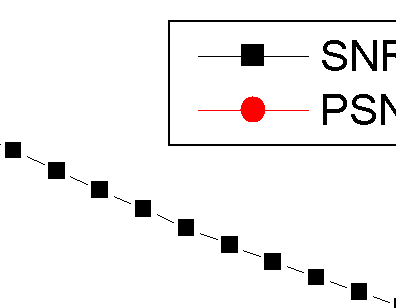
\includegraphics[width=\ww\linewidth]{obraz1}}
\hfill%
\subfloat[GIF]{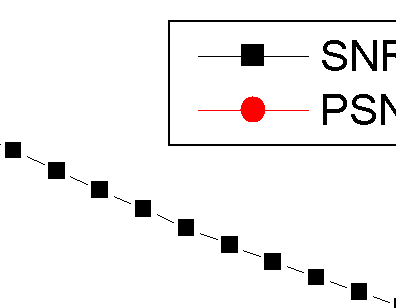
\includegraphics[width=\ww\linewidth]{obraz1_gif}} 
\hfill% wypełnenie
\subfloat[JPG: q=1]{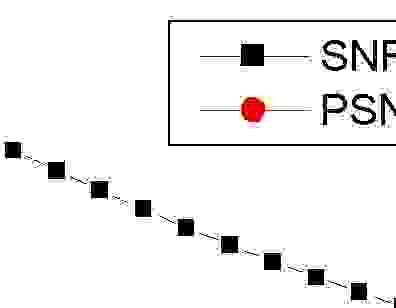
\includegraphics[width=\ww\linewidth]{obraz1_q=1.jpg}}
\hfill
\subfloat[JPG: q=80]{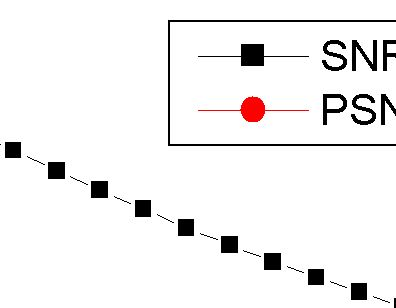
\includegraphics[width=\ww\linewidth]{obraz1_q=80.jpg}}
\hfill%
\subfloat[JP2: Q=8]{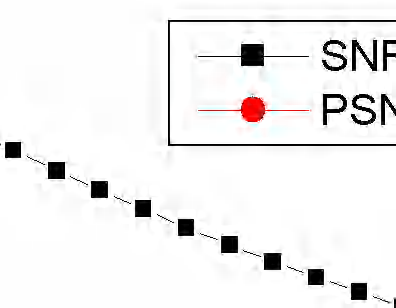
\includegraphics[width=\ww\linewidth]{obraz1_Q=8_jp2}}
\hfill%
\subfloat[JP2: Q=30]{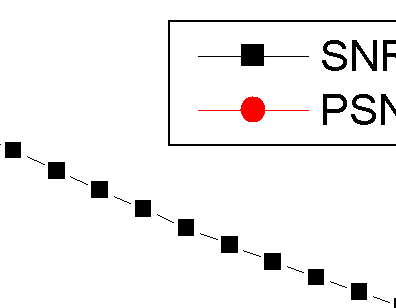
\includegraphics[width=\ww\linewidth]{obraz1_Q=30_jp2}}
\caption{Porównanie metod kompresji dla obrazu syntetycznego} %
\label{fig:porownanie2}
\end{figure}

%Zwróccie uwagę na to, że w obu przypadkach jakość grafik nie ulega degradacji.


\end{document}